\documentclass[number=03]{assignment}
\title{Computer Architecture - TE2031}
\chead{Assignment 04}
\rhead{MIPS building blocks}
%\date{February - June 2020}

\newif\ifanswers
\answerstrue % comment out to hide answers

\newcommand{\alupkgfile}{\colorfilename{mips\_pkg.sv}}
\newcommand{\alufile}{\colorfilename{alu.sv}}
\newcommand{\tbalufile}{\colorfilename{tb\_alu.sv}}
\newcommand{\sgnextfile}{\colorfilename{sgn\_ext.sv}}
\newcommand{\tbsgnextfile}{\colorfilename{tb\_sgn\_ext.sv}}

\newcommand{\rfpkgfile}{\colorfilename{mips\_pkg.sv}}
\newcommand{\rffile}{\colorfilename{rf.sv}}
\newcommand{\tbrffile}{\colorfilename{tb\_rf.sv}}
\newcommand{\dorffile}{\colorfilename{rf.do}}

\newcommand{\imfile}{\colorfilename{im.sv}}
\newcommand{\tbimfile}{\colorfilename{tb\_im.sv}}

\newcommand{\dmfile}{\colorfilename{dm.sv}}
\newcommand{\tbdmfile}{\colorfilename{tb\_dm.sv}}

\newcommand{\dofile}{\colorfilename{mips.do}}

\newcommand{\deadline}{23:59 hours on Wednesday September 30th 2020}
\makesavenoteenv{tabular}
\makesavenoteenv{table}
% Begin document
\begin{document}

\setcounter{chapter}{1}
\chapter*{Assignment 04 \\ MIPS building blocks}
% ======================================
% Objective
% ======================================
\section{Objectives}
To design and test the basic \ac{MIPS} building blocks using \SV.
\begin{enumerate}
\item To design and test an \ac{ALU} using \SV. 
\item To design and test a sign extender using \SV.
\item To design and test a \ac{RF} using \SV.
\item To design and test an \ac{IM} using \SV. 
\item To design and test a \ac{DM} using \SV. 
\end{enumerate}

% ======================================
% Deadline
% ======================================
\section{Deadline}
\alertblue{\deadline.}
% ======================================
% Teamwork policy
% ======================================
\section{Teamwork policy}
This is an individual assignment. 
% ======================================
% Pre-requisites
% ======================================
\section{Pre-requisites}
It is assumed that you are familiar with working with \ModelSim and \Quartus. 
If you require assistance, you can refer to the first assignment tutorial.
% ======================================
% Background
% ======================================
\section{Background}
The following sections provide some background to the designs for this assignment.

\acresetall
% ======================================
% ALU
% ====================================== 
\subsection{\acs{ALU}}\label{sec:ALU_background}
An \ac{ALU} is the component of a \ac{uP} that performs the most basic arithmetic and logical operations.
The schematic symbol of an \ac{ALU} is shown in \fref{Figure:ALU}.
%
\begin{figure}[!ht]
\centering
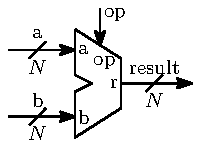
\includegraphics[scale=1.5]{ALU}
\caption{\ac{ALU} schematic symbol.}
\label{Figure:ALU}
\end{figure}
%
\newpage 
In \fref{Figure:ALU}, the \ac{ALU} receives two $N$-bit operands, \code{a} and \code{b}, as well as a signal \code{op}, which indicates the type of operation the \ac{ALU} must perform. 
More specifically, the value of \code{op} specifies whether the \ac{ALU} should perform an addition, a subtraction or any bitwise logical operation such as \code{AND}, \code{OR}, \code{XOR}, \emph{etc}, between the two input operands.
The \ac{ALU} delivers an $N$-bit output, labelled as \code{result} in \fref{Figure:ALU}, which corresponds to the result of the arithmetic or logical operation.

% ======================================
% Sign extender
% ====================================== 
\subsection{Sign extender}\label{sec:SgnExt_background}
A sign extender is a basic building block of a \ac{uP} that takes an $N$-bit input \code{data\_in} and generates an $M$-bit output \code{data\_out}, as shown in \fref{Figure:sgn_ext}.
%
\begin{figure}[!h]
\centering
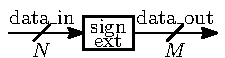
\includegraphics[scale=2.0]{sgn_ext}
\caption{Sign extender schematic symbol.}
\label{Figure:sgn_ext}
\end{figure}
%

Here, it is assumed that $N < M$.
A sign extender increases the number of bits of a signed number while preserving the number's sign.
This is achieved by replicating the sign bit, the \ac{MSB} in 2's complement, of \code{data\_in} $(M-N)$ times and then appending these replicated bits as its \acp{MSB}.
For example, assume that $N=5$ and $M=8$.
Here, the sign extender must generate an $8$-bit output \code{data\_out} from a $5$-bit input \code{data\_in}. 
In order to achieve this, this blocks replicates the sign bit of \code{data\_in} $(M-N)=(8-5)=3$ times.
Furthermore, if \code{data\_in = 5'b11000}, representing the decimal number $-8$ in 2's complement, its $8$-bit sign-extended version corresponds to \code{data\_out = 8'b\textcolor{blue}{111}10000}, which also corresponds to the decimal value $-8$.

One important aspect of this block is that it must preserve the sign of the input data and not only increase the number of bits by doing zero-padding. 
This may lead to an erroneous result.
Consider the same scenario as above, with $N=5$ and $M=8$ and \code{data\_in = 5'b11000}, representing decimal number $-8$.
If we carelessly increase the number of bits from $5$ to $8$ by adding zeros, then we will generate \code{data\_in = 8'b\textcolor{blue}{000}11000}, which corresponds to decimal value $+24$, rather than the expected value of $-8$.

% ======================================
% Register file
% ====================================== 
\subsection{Register File}
One of the main characteristics of a \ac{RISC} \ac{ISA} is the load-store approach. 
This implies that all operands used in the \ac{ALU} must be retrieved from a register source instead of main memory.
A \ac{RF} is simply a collection of registers, or memory elements, in which any register may be written to or read from at any clock cycle.
There are 32 registers in \ac{MIPS} \ac{ISA}, some of which are used to store the status of the \ac{uP} and some other to store temporary data used by the user program.
\fref{Figure:RF_schematic} shows the schematic symbol of a simple \ac{RF} that may be used in a \ac{MIPS} \ac{uP}.
%
\begin{figure}[!ht]
\centering
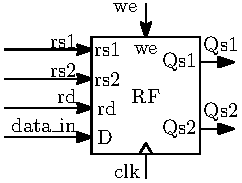
\includegraphics[scale=1.5]{RegFile_schematic}
\caption{\ac{RF} schematic symbol.}
\label{Figure:RF_schematic}
\end{figure}
%

The \ac{RF} of \fref{Figure:RF_schematic} outputs \code{Qs1} and \code{Qs2}, which are the contents of the two read register \code{rs1} and \code{rs2}, respectively. 
These reads are performed at any given time.
However, writes of input \code{data\_in} in write address \code{rd} are controlled by the write enable control signal \code{we}, which must be asserted for a write to occur at the clock edge determined by \code{clk}.

% ======================================
% Instruction Memory
% ====================================== 
\subsection{Instruction Memory}
As its name suggests, an \ac{IM} stores the instructions to be performed by the \ac{MIPS}. 
This memory is a \ac{ROM}, whose values are initialized by the programmer prior the execution of the very first instruction by the \ac{MIPS}. 
\fref{Figure:IM} shows the schematic symbol of an \ac{IM}.
%
\begin{figure}[!ht]
\centering
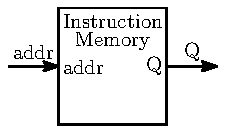
\includegraphics[scale=1.5]{MIPS_design_IM}
\caption{\ac{IM} schematic symbol.}
\label{Figure:IM}
\end{figure}
%

Here, output \code{Q} outputs the data stored in memory address \code{addr}.


% ======================================
% Data Memory
% ====================================== 
\subsection{Data Memory}
As its name suggests, a \ac{DM} stores temporary data used by the user program.
\ac{DM} is basically a \ac{RAM} whose values are read/written according to the user program.
\fref{Figure:DM} shows the schematic symbol of an \ac{DM}.
%
\begin{figure}[!ht]
\centering
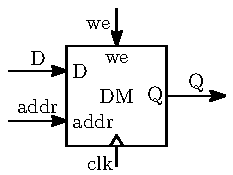
\includegraphics[scale=1.5]{MIPS_design_DM}
\caption{\ac{DM} schematic symbol.}
\label{Figure:DM}
\end{figure}
%
\newpage 
Here, \code{we} is a control signal that enables writes into the memory. 
More specifically, if \code{we} is asserted to logic 1, the input data \code{D} will be stored in address \code{addr} at the rising edge of \code{clk}.
If \code{we} has the value of 0, input data \code{D} will be ignored.
Output \code{Q} outputs the data stored in memory address \code{addr} and it is not dependant on \code{we} or \code{clk}.

% ======================================
% Specifications
% ======================================
\section{Design specifications}
The following sections describe the specifications for all the required \ac{MIPS} building blocks.
Please make sure you use the names provided in the specifications for both the file names and the ports of each module.

% ======================================
% ALU specs
% ====================================== 
\subsection{\acs{ALU}}\label{sec:ALU_specs}
Your \ac{ALU} design must be done in a \SV file named \alufile, which must contain a \module named \code{alu} and the port definition of \tref{Table:ALU_ports}.
For this assignment, assume a value of \code{DATA\_WIDTH=16}.
However, bear in mind that your \ac{ALU} design \alertred{must} be able to correctly perform all operations regardless of the value assign to the \parameter \code{DATA\_WIDTH}. 
This \parameter must be declared in a \SV \package named \alupkgfile.

%
\begin{table}[!htb]
\centering
\caption{\acs{ALU} ports.}
\label{Table:ALU_ports}
\begin{threeparttable}
\begin{tabular}{l|l|l|c|l}
\hline\hline
Port name & Direction & Data type & Width & Description \\
\hline\hline
\code{a}          & \code{input} & logic signed   & \code{DATA\_WIDTH} & Operand a. \\ \hline
\code{b}          & \code{input} & logic signed   & \code{DATA\_WIDTH} & Operand b. \\ \hline  
\code{op}         & \code{input} & \code{alu\_op\_t} & -\tnote{\alertblue{*}} & Operation to be performed. \\ \hline  
\multirow{2}{*}{\code{result}}     & \multirow{2}{*}{\code{output}} & \multirow{2}{*}{logic signed}    & \multirow{2}{*}{\code{DATA\_WIDTH}} & Result from the arithmetic \\
 & & & & or logical operation. \\ \hline 
\multirow{2}{*}{\code{zero}}          & \multirow{2}{*}{\code{output}} & \multirow{2}{*}{logic}    & \multirow{2}{*}{\code{1}} & Zero flag. Active high when \\
 & & & & result is exactly zero. \\ \hline
\multirow{2}{*}{\code{neg}}          & \multirow{2}{*}{\code{output}} & \multirow{2}{*}{logic}    & \multirow{2}{*}{\code{1}} & Negative flag. Active high when \\
 & & & & result is negative. \\ \hline
\multirow{2}{*}{\code{grt}}          & \multirow{2}{*}{\code{output}} & \multirow{2}{*}{logic}    & \multirow{2}{*}{\code{1}} & Greater-than flag. Active high when \\
 & & & & \code{a} is greater than \code{b}. \\ \hline
 \multirow{2}{*}{\code{eq}}          & \multirow{2}{*}{\code{output}} & \multirow{2}{*}{logic}    & \multirow{2}{*}{\code{1}} & Equal flag. Active high when \\
 & & & & \code{a} and \code{b} have the same value. \\ \hline
\hline
\end{tabular}
\begin{tablenotes}\footnotesize
\item[\alertblue{*}] There's no need to specify the width of this port. This data type is specified in \alupkgfile.
\end{tablenotes}
\end{threeparttable}
\end{table}
%

The operations that the \ac{ALU} must perform are described in \tref{Table:ALU_operations}.
These operations must be defined in a user-defined \enum data type named \code{alu\_op\_t} and declared in a \SV \package named \alupkgfile.
Moreover, \tref{Table:ALU_operations} specifies the name of the \enum you must use for the different \ac{ALU} operations.

%
\begin{table}[!htb]
\centering
\caption{\acs{ALU} operations.}
\label{Table:ALU_operations}
\begin{tabular}{l|l|l}
\hline\hline
 Operation type & Enum name & Meaning \\
 \hline\hline
 \multirow{2}{*}{Arithmetic} & \code{ALU\_ADD} & Addition    \\
                             & \code{ALU\_SUB} & Subtraction \\
                                                         \hline
 \multirow{6}{*}{Logical} & \code{ALU\_NAND} & Logical NAND \\
                          & \code{ALU\_NOR}  & Logical NOR  \\
                          & \code{ALU\_XNOR} & Logical XNOR \\
                          & \code{ALU\_AND} & Logical AND   \\
                          & \code{ALU\_OR}  & Logical OR    \\
                          & \code{ALU\_XOR} & Logical XOR   \\
                          \hline
 \multirow{4}{*}{Shift} & \code{ALU\_SLL} & Shift left logical \\
                             & \code{ALU\_SRL} & Shift right logical \\
                             & \code{ALU\_SLA} & Shift left arithmetic \\
                             & \code{ALU\_SRA} & Shift right arithmetic \\
                             \hline
 \multirow{2}{*}{Load with immediate} & \code{ALU\_LUI} & Load upper with immediate \\
                                      & \code{ALU\_LLI} & Load lower with immediate  \\
                             \hline
Comparison & \code{ALU\_CMP} & Compares \code{a} and \code{b} \\ 
 \hline\hline
 \end{tabular}
\end{table}
%

It is important to note that \code{zero}, \code{neg}, \code{grt} and \code{eq} flags of \tref{Table:ALU_ports} must be updated for every operation of \tref{Table:ALU_operations}.
More specifically, these outputs must be calculated for each of the 15 different \ac{ALU} operations.
The following sections provide some information about each type of operation of \tref{Table:ALU_operations}

\subsubsection{Arithmetic operations}
Arithmetic operations must be performed over signed operands.

\subsubsection{Logical operations}
All logical operations are bitwise operations.

\subsubsection{Shift operations}
Operand \code{a} indicates the shift amount for \code{b}.
For example, assume the following scenarios. 
%
\begin{table}[!htb]
\centering
\caption{\acs{ALU} shift operations example.}
\label{Table:ALU_shifts}
\begin{tabular}{c|c|c|c|c|c|c|c}
\hline\hline
\code{op} & \code{a} & \code{b} & \code{result} & \code{zero} & \code{neg} & \code{grt} & \code{eq} \\
\hline\hline
\code{ALU\_SLL} & \code{16'h0004} & \code{16'hFEDC} & \code{16'hEDC0} & \code{0} & \code{1} & \code{1} & \code{0} \\
\hline
\code{ALU\_SRA} & \code{16'h0004} & \code{16'hFEDC} & \code{16'hFFED} & \code{0} & \code{1} & \code{1} & \code{0} \\
\hline
 \end{tabular}
\end{table}
%

\subsubsection{Load with immediate operations}
The lower half of operand \code{b}, \ie bits \code{[DATA\_WIDTH/2-1:0]}, are used to load the upper or lower part of the output \code{result}. 
The other half of \code{result} must be padded with zeros.
For example, assume \code{DATA\_WIDTH=16}. 
In this scenario, \code{result} is calculated as follows.
\begin{itemize}
\item[] \code{ALU\_LUI: result = \{b[7:0],8'b0\}}
\item[] \code{ALU\_LLI: result = \{8'b0,b[7:0]\}}
\end{itemize}

\tref{Table:ALU_load} provides a more thorough example of load with immediate operations considering all \ac{ALU} inputs and outputs.
Here, note that the value of operand \code{a} is only relevant for the flags.
%
\begin{table}[!htb]
\centering
\caption{\acs{ALU} load operations.}
\label{Table:ALU_load}
\begin{tabular}{c|c|c|c|c|c|c|c}
\hline\hline
\code{op} & \code{a} & \code{b} & \code{result} & \code{zero} & \code{neg} & \code{grt} & \code{eq} \\
\hline\hline
\code{ALU\_LUI} & \code{16'h0000} & \code{16'hFEDC} & \code{16'hDC00} & \code{0} & \code{1} & \code{1} & \code{0} \\
\hline
\code{ALU\_LLI} & \code{16'h8888} & \code{16'hFEDC} & \code{16'h00DC} & \code{0} & \code{0} & \code{0} & \code{0} \\
\hline
\end{tabular}
\end{table}
%

\subsubsection{Comparison}
Output \code{result} must be set to 0 and all the flags must be updated accordingly.
For example, assume the following scenarios.
%
\begin{table}[!htb]
\centering
\caption{\acs{ALU} comparison operation example.}
\label{Table:ALU_compare}
\begin{tabular}{c|c|c|c|c|c|c|c}
\hline\hline
\code{op} & \code{a} & \code{b} & \code{result} & \code{zero} & \code{neg} & \code{grt} & \code{eq} \\
\hline\hline
\code{ALU\_CMP} & \code{4} & \code{-3} & \code{0} & \code{1} & \code{0} & \code{1} & \code{0} \\
\hline
\code{ALU\_CMP} & \code{-1} & \code{-1} & \code{0} & \code{1} & \code{0} & \code{0} & \code{1} \\
\hline
\code{ALU\_CMP} & \code{-7} & \code{0} & \code{0} & \code{1} & \code{0} & \code{0} & \code{0} \\
\hline
\end{tabular}
\end{table}
%
\newpage
% ======================================
% Sign extender specs
% ====================================== 
\subsection{Sign extender}\label{sec:SgnExt_specs}
Your sign extender design must be done in a \SV file named \sgnextfile, which must contain a \module named \code{sgn\_ext} and the port definition of \tref{Table:sgn_ext_ports}.
%
\begin{table}[!ht]
\centering
\caption{Sign extender ports.}
\label{Table:sgn_ext_ports}
\begin{tabular}{l|l|l|c|l}
\hline\hline
Port name & Direction & Data type & Width & Description \\
\hline\hline
\multirow{2}{*}{\code{sign}}          & \multirow{2}{*}{\code{input}}  & \multirow{2}{*}{logic} & \multirow{2}{*}{\code{1}}  & Determines whether \code{data\_in} \\ 
& & & & should be sign- or zero-extended.               \\ \hline
\code{data\_in}          & \code{input}  & logic & \code{DATA\_WIDTH\_IN}  & Input data.               \\ \hline
\code{data\_out}         & \code{output} & logic & \code{DATA\_WIDTH\_OUT} & Sign-extended output data. \\ \hline  
\hline
\end{tabular}
\end{table}
%

Parameters \code{DATA\_WIDTH\_IN} and \code{DATA\_WIDTH\_OUT} must be included as part of the \module declaration and not in \alupkgfile.

Note that in contrast to the sign extender described in \sref{sec:SgnExt_background}, you are required to include the option to perform zero-extension.
This will be achieved by the input signal \code{sign}.
More specifically, if input \code{sign = 1}, output \code{data\_out} should be sign-extended.
By contrast, if input \code{sign = 0}, \code{output data\_out} should be zero-extended. 
For example, assume the following scenarios for the case when \code{DATA\_WIDTH\_IN = 4} and \code{DATA\_WIDTH\_OUT = 8}.
%
\begin{table}[!h]
\centering
\caption{Sign extender operation example.}
\label{Table:Sign_extender_example}
\begin{tabular}{c|c|c}
\hline\hline
\code{sign} & \code{data\_in} & \code{data\_out}  \\
\hline\hline
\code{0} & \code{4'h8} & \code{8'h08} \\ \hline
\code{0} & \code{4'h7} & \code{8'h07} \\ \hline
\code{1} & \code{4'h8} & \code{8'hF8} \\ \hline
\code{1} & \code{4'h7} & \code{8'h07} \\ \hline
\hline
\end{tabular}
\end{table}
%

\subsection{Register File}
Your \ac{RF} design must be described in a \SV file named \rffile, which must contain a \module named \code{rf} and the port definition of \tref{Table:rf_ports}.
For this assignment, assume a value of \code{DATA\_WIDTH=16} and \code{RF\_N\_WORDS=32}.
However, bear in mind that your design \alertred{must} be able read/write data from/to the \ac{RF} correctly regardless of the number of addresses or the width of the input data.
These \parameter must be declared in the \rfpkgfile.

%
\begin{table}[!htb]
\centering
\caption{\acl{RF} ports.}
\label{Table:rf_ports}
\begin{threeparttable}
\begin{tabular}{l|l|l|c|l}
\hline\hline
Port name & Direction & Data type & Width & Description \\
\hline\hline
\code{clk}          & \code{input}  & logic & 1 & Clock \\ \hline
\code{asyn\_n\_rst} & \code{input}  & logic & 1 & Active-low asynchronous  reset \\ \hline
\code{we}           & \code{input}  & logic & 1 & Write enable \\\hline
\code{rs1}          & \code{input}  & logic & \code{RF\_ADDRESS\_WIDTH}\tnote{\alertblue{*}} & First read address\\ \hline
\code{rs2}          & \code{input}  & logic & \code{RF\_ADDRESS\_WIDTH}\tnote{\alertblue{*}} & Second read address \\ \hline  
\code{rd}           & \code{input}  & logic & \code{RF\_ADDRESS\_WIDTH}\tnote{\alertblue{*}} & Write address \\ \hline  
\code{data\_in}     & \code{input}  & logic & \code{DATA\_WIDTH} & Data to be stored \\\hline
\code{Qs1}          & \code{output} & logic & \code{DATA\_WIDTH} & Data from read from \code{rs1} \\\hline
\code{Qs2}          & \code{output} & logic & \code{DATA\_WIDTH} & Data from read from \code{rs2} \\\hline
\hline
\end{tabular}
\begin{tablenotes}\footnotesize
\item[\alertblue{*}] \code{RF\_ADDRESS\_WIDTH=$\lceil\log_{2}$(RF\_N\_WORDS)$\rceil$}
\end{tablenotes}
\end{threeparttable}
\end{table}
%
\newpage
Note that \code{asyn\_n\_rst} input of  \tref{Table:rf_ports} is not depicted in \fref{Figure:RF_schematic} for simplification purposes only.

\subsection{Instruction Memory}
Your \ac{IM} design must be described in a \SV file named \imfile, which must contain a \module named \code{im} and the port definition of  
\tref{Table:im_ports}. 
%
\begin{table}[!htb]
\centering
\caption{\acl{IM} ports.}
\label{Table:im_ports}
\begin{threeparttable}
\begin{tabular}{l|l|l|c|l}
\hline\hline
Port name & Direction & Data type & Width & Description \\
\hline\hline
\code{init\_file}          & -  & parameter & - & Name of \ac{IM} initialization file.\\ \hline
\code{addr}          & \code{input}  & logic & \code{IM\_ADDRESS\_WIDTH}\tnote{\alertblue{*}} & Read address\\ \hline
\code{Q}          & \code{output} & logic & \code{INSTRUCTION\_WIDTH} & Data from read from \code{addr} \\\hline
\hline
\end{tabular}
\begin{tablenotes}\footnotesize
\item[\alertblue{*}] \code{IM\_ADDRESS\_WIDTH=$\lceil\log_{2}$(IM\_N\_WORDS)$\rceil$}
\end{tablenotes}
\end{threeparttable}
\end{table}
%

For this assignment, you may use \code{INSTRUCTION\_WIDTH=32} and \code{IM\_N\_WORDS=64}.
However, bear in mind that your design \alertred{must} be parameterizable and able read data from the \ac{IM} correctly regardless of the number of addresses or the width of data stored in the memory.
These \parameter must be declared in the \rfpkgfile.

\alertblack{HINT.} Your \ac{IM} design must initialize the contents of the memory by loading a text file defined in module parameter \code{init\_file}. For this purpose, you may like to investigate the \SV directives \code{\$readmemb} and \code{\$readmemh}.

\subsection{Data Memory}
Your \ac{DM} design must be described in a \SV file named \dmfile, which must contain a \module named \code{dm} and the port definition of  
\tref{Table:dm_ports}. 
%
\begin{table}[!htb]
\centering
\caption{\acl{DM} ports.}
\label{Table:dm_ports}
\begin{threeparttable}
\begin{tabular}{l|l|l|c|l}
\hline\hline
Port name & Direction & Data type & Width & Description \\
\hline\hline
\code{clk}          & \code{input}  & logic & 1 & Clock\\ \hline
\code{we}           & \code{input}  & logic & 1 & Write enable \\\hline
\code{D}            & \code{input}  & logic & \code{DATA\_WIDTH} & Data input \\\hline
\code{addr}         & \code{input}  & logic & \code{DM\_ADDRESS\_WIDTH}\tnote{\alertblue{*}} & Read address\\ \hline
\code{Q}          & \code{output} & logic & \code{DATA\_WIDTH} & Data from read from \code{addr} \\\hline
\hline
\end{tabular}
\begin{tablenotes}\footnotesize
\item[\alertblue{*}] \code{DM\_ADDRESS\_WIDTH=$\lceil\log_{2}$(DM\_N\_WORDS)$\rceil$}
\end{tablenotes}
\end{threeparttable}
\end{table}

For this assignment, you may use \code{DATA\_WIDTH=16} and \code{DM\_N\_WORDS=64}.
However, bear in mind that your design \alertred{must} be parameterizable and able read/write data from/to the \ac{DM} correctly regardless of the number of addresses or data width.
These \parameter must be declared in the \rfpkgfile.

\alertblack{HINT.} Your \ac{DM} does not require a reset signal. As a result of this, you may simply initialize the \ac{DM} contents directly in your testbench.

% ======================================
% Grading criteria
% ====================================== 
\section{Grading criteria}\label{sec:Grading}
For this assignment, I will consider the following grading criteria.
\begin{enumerate}
\item \alertblue{The correct functionality of your designs.}
I will use my own testbenches in order to automatically stress your designs and verify that they perform the tasks according to the specifications. 
For example, I will try different values for the parameters in your designs and I expect them to still perform according to the specifications.
This is why it is paramount that you follow the name convention specified for file names and port names.
Moreover, it is important that your designs and testbenches compile in \ModelSim without errors.
\alertred{Your maximum grade for this assignment will automatically drop to 50/100 should \ModelSim trigger a compilation or simulation error.}
\item \alertblue{The quality of your testbenches.}
Even though I will use my own testbenches, I expect you to consider a thorough and concious set of test scenarios.
In this way, you should be able to spot any mismatches between the expected results and the actual results provided by your designs.
\item \alertblue{Your designs must be synthesized in \Quartus without latches and without errors.}
Warnings are tolerated at this point.
\alertred{Your maximum grade for this assignment will automatically drop to 50/100 should \Quartus trigger a synthesis error or generate unwanted latches.}
Remember that a design is not useful if it can't be synthesized.
\end{enumerate}


% ======================================
% Deliverables and Submission instructions
% ====================================== 
\section{Deliverables and Submission instructions}\label{sec:Deliverables}
Prepare a single \code{zip} file containing the following files.
\begin{enumerate}
\item \alupkgfile.
\item \alufile.
\item \sgnextfile.
\item \rffile.
\item \imfile.
\item \dmfile.
\item \tbalufile.
\item \tbsgnextfile.
\item \tbrffile.
\item \tbimfile.
\item \tbdmfile.
\item A \code{.do} script for compiling and simulating any of the building blocks listed above.
\end{enumerate}

Submit your assignment through Canvas \alertred{no later} than \deadline. 
\\
Please send any questions to \href{mailto:isaac.perez.andrade@tec.mx}{isaac.perez.andrade@tec.mx}.
\end{document}
